\subsection{The concept of machine learning}

For many decades computers have been an integral aspect of science, handling large amounts of data, completing tedious calculations and controlling experiments. For the most part the  machines were assigned discrete tasks. They step-wise followed commands previously designed by human users and with non statistical outcomes. 
For particle physics in particular computers were used to select interesting data from large samples when given proper instructions making it possible to process amounts of data that would have exceeded human capacities. However the selection rules had always to be generated by the user, therefore requiring an in depth analysis of the underlying system. Artificial intelligence presents a way for a program to establish its own decision rules and improve these over several iterations and thereby learning to solve the problem all by itself.\\
There has been a great effort over the last decades trying to implement a way for machines to learn from experience and thereby enable them to analyse complex tasks in a wide range of applications.\\
Often times the human understanding of the task and the work done by the machine itself are in equilibrium as great knowledge of an assignment is required to find the most efficient way to have a machine not only work on it but work on it efficiently. This means fine tuning the machine's capabilities and degrees of freedom to the requirements and is called hyperparameter optimisation.\\
The task of machine learning can be simplified by comparing what a living being needs to be able to learn solving new problems, which can be split into understanding a system, evaluating a decision step and generating new decision steps.\\
Understanding a system means when given a task having a way to observe all features and possibilities relevant to work on the task. Humans have their senses to easily break down their observations into useful features and concepts that can then be processed for decision making. A computer has no senses built in and for most tasks this means that the step of filtering information for a relevant subset of features has still to be done by humans or a good preprocessing algorithm.\\
Once a system has been converted to a subset of features usable by a computer the step of making own decisions has to be implemented. This can be done by weighting and interconnecting the information using structures often times inspired by the structure of the neurons in the human brain.\\
This process of decision making at the basis is somewhat random and so far no way of evaluating the success of a decision rule has been introduced. This is where a cost function comes into play.It pairs a generated decision rule with an estimator of its quality. Combined with an optimiser which suggests further steps, this function is a basis for a network to independently approach a good decision rule for a somewhat un-investigated topic.\\
A very commonly used machine learning algorithm is the artificial neural network which on its own forms a quite broad field that builds the base of this work. The most important concepts of machine learning will be explained using the example of a neural network. For the explanation of input, decision making process and the generation of a gradient the example of a neural network will be used.

\subsection{Neural Networks}

The artificial neural network, or just neural network, is the most commonly known approach to machine learning. Its structure is inspired by the neurons forming the human brain which is also where it gets its name from.\\
Instead of neurons a neural network consists of numerous very simple processors, called nodes. These nodes are usually structured into several layers. As presented in fig (todo). Also there is several ways to structure and connect these nodes often times matching a certain problem in this explanation only the most commonly way is explained. In that case each node of a layer is getting input from each node in the last layer and is outputting to each node of the following layer. Such a network structure is shown in figure \ref{fig:nodes_nomenclature}. It describes the step between a node and the previous layer. The math will be explained in detail later.

\begin{figure}
	\centering
	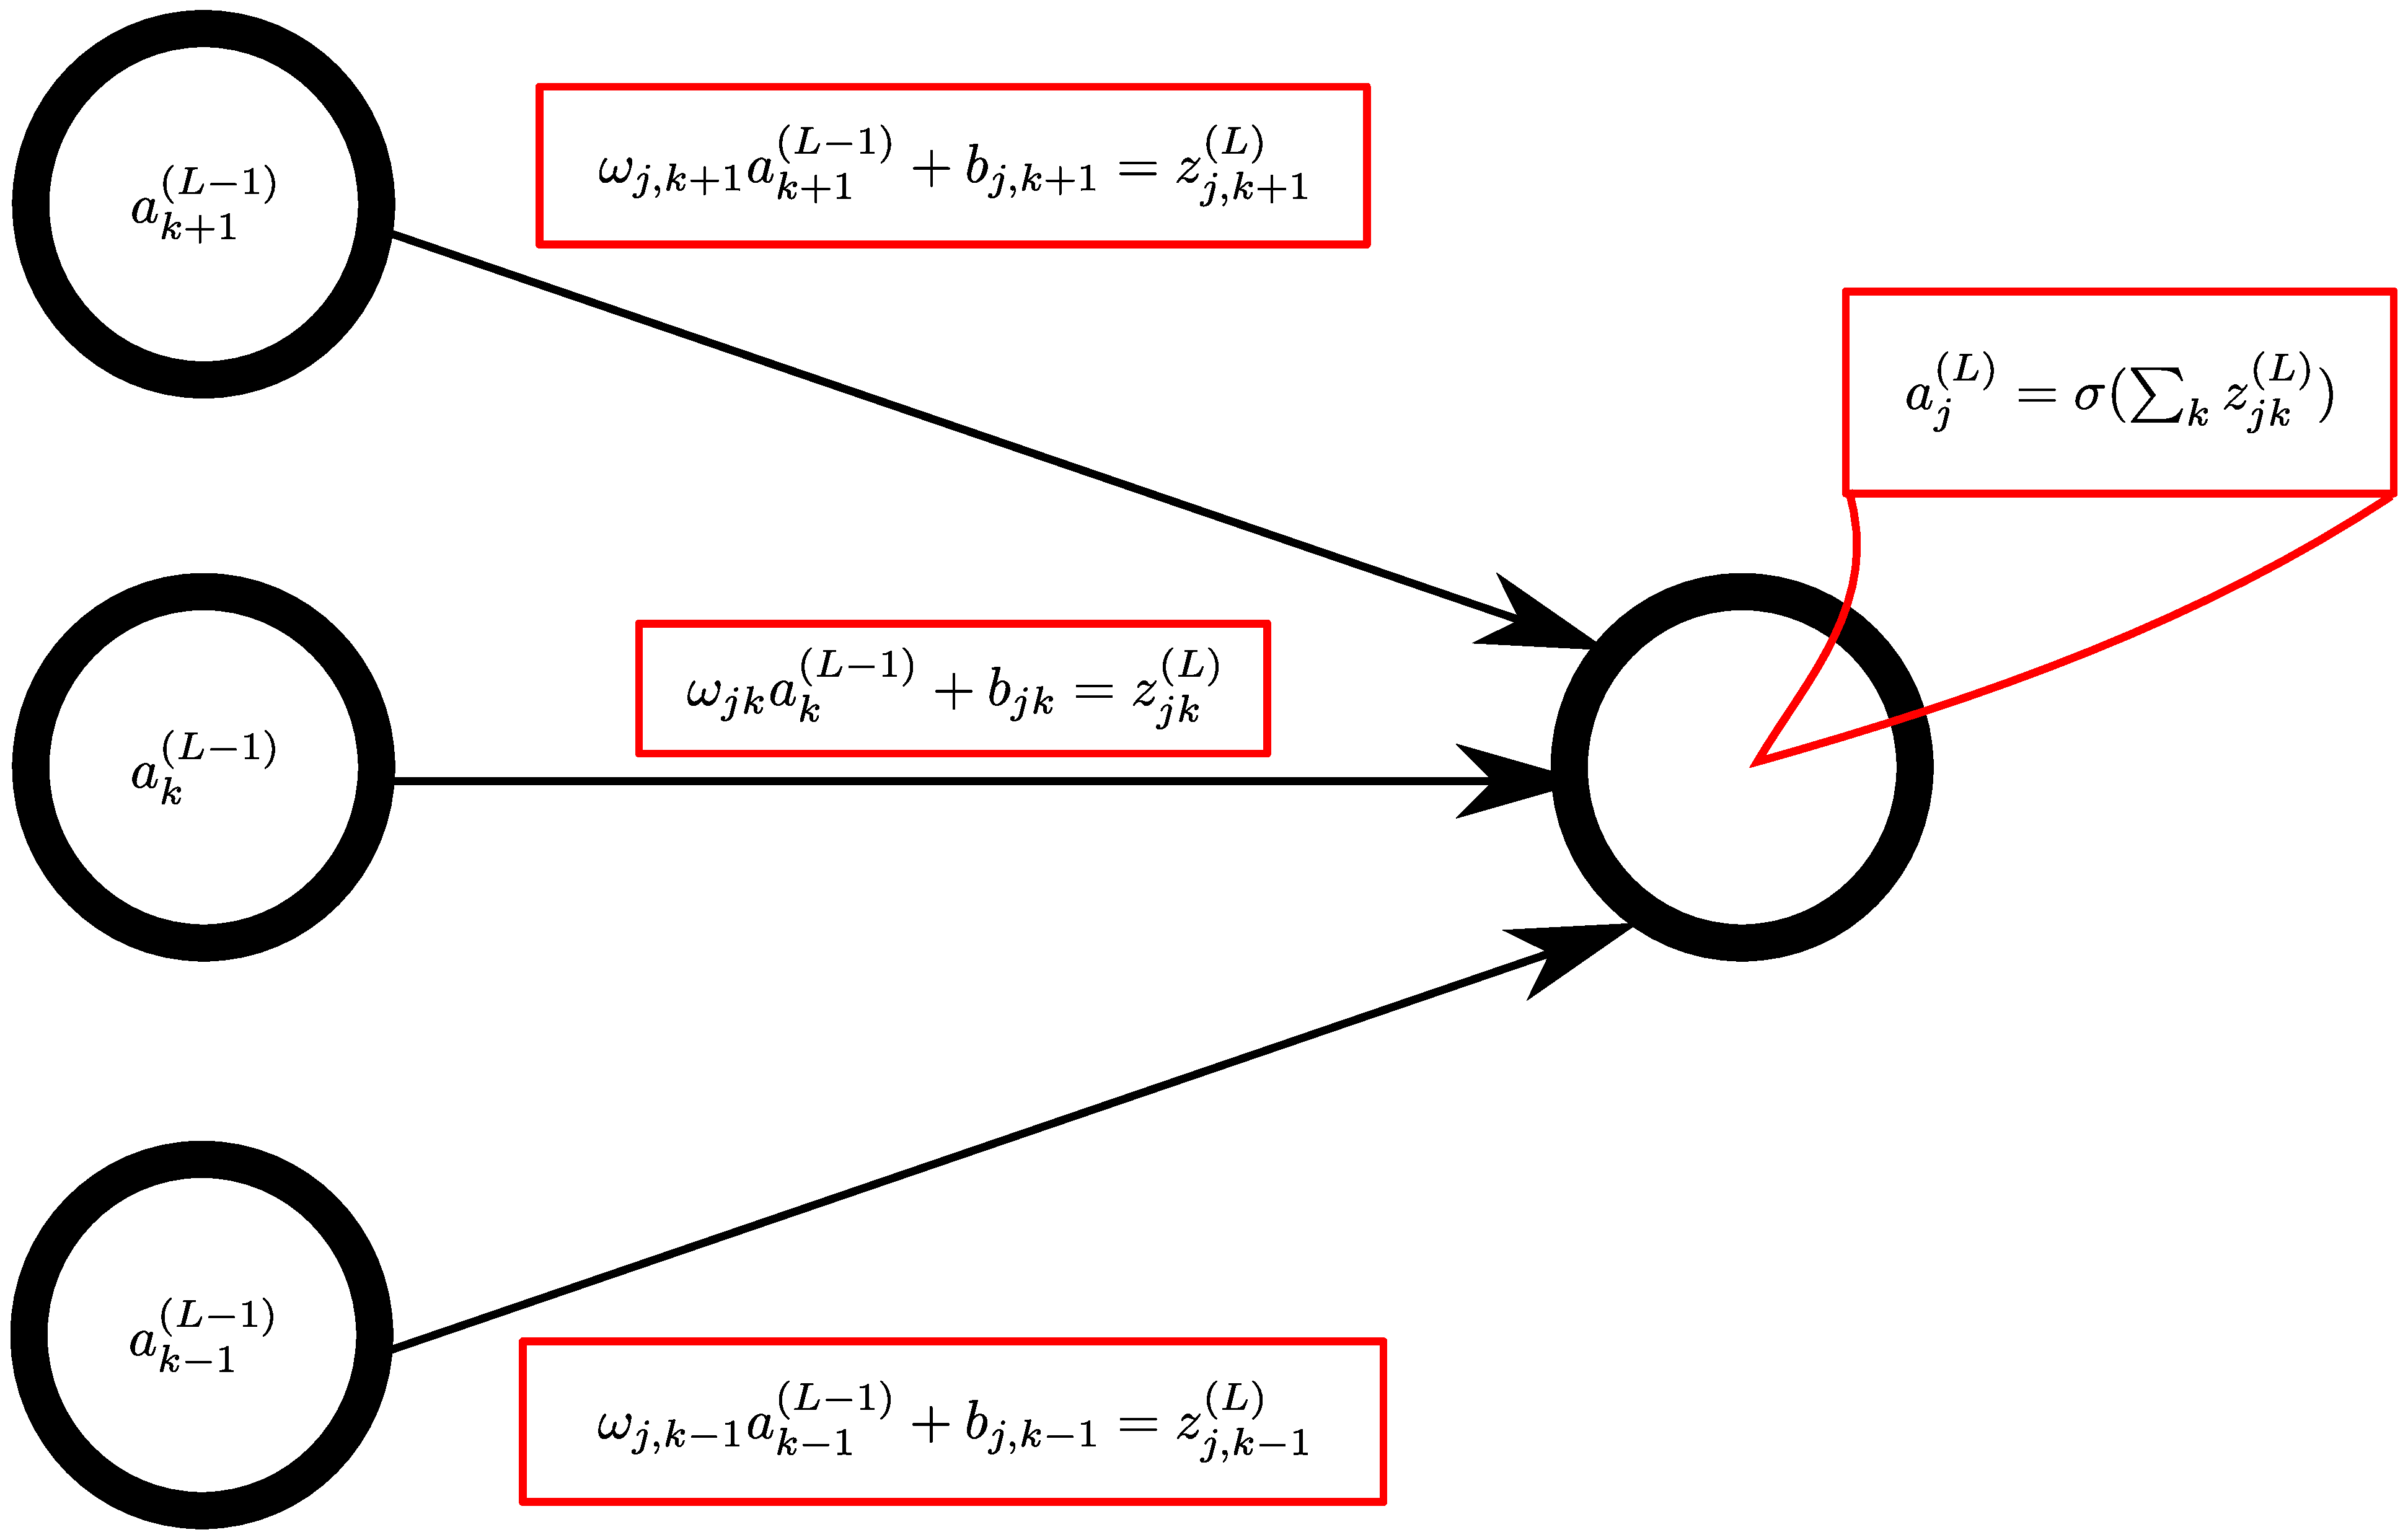
\includegraphics[scale=0.18]{figures_ML/nodes_nomenclature.eps}
	\caption{Network propagation from layer $(L-1)$ to layer $L$}
	\label{fig:nodes_nomenclature}
\end{figure}


\subsubsection{The input layer}

To understand a task and draw reasonable conclusions first the underlying system has to be understood. Its features need to be found and summarised. The human brain is capable of investigate unknown systems and learn the features that are the most unique or interesting. For that it has its senses to explore the system and process them later. To allow a machine to do something similar the unknown system has to be represented in a way that it is clear for the network what to look out for. This is usually the task that needs the most preprocessing by the user. The simplest case is to submit a list of variables to the network. In particle physics this could be kinematic variables of the particles in an event.
The input to a neural network is just given to the input layer of nodes and then processed through each following layer. For different tasks different layers might deal with different parts of the information but in this work the linear way of giving all information used to an input layer and then processing it is used.

\subsubsection{Decision making process}

Computers being not much more than very powerful calculators, excel at performing high numbers of clearly defined calculations. The trick is that the task has to be defined clearly. There usually is no fuzziness.\\
This is very different for the human brain. We rely on a certain fuzziness when processing information through a net of neurons where the output of every neuron is taken as input for the surrounding neurons. The challenge of machine learning is to represent this fuzziness by many somewhat discrete calculations. In the neural network the neurons and their fuzzy interaction is represented by the nodes which are very simple processors. Like neurons each node can use input from many other nodes to create a new output signal. Thereby the input information can be linked to each other in numerous ways. Combined with weights this allows for were clear decisions made from a complex set of input information.\\
The input of every node is the weighted output of all previous nodes as shown in equation \eqref{eq:node_input}. $z_j^L$ is the input to the $j$-th in the $L$-th layer. $\omega_{jk}^L$ is the weight from the $k$-th node in the previous layer to the node, $a_k^{L-1}$ is the nodes output and $b_k$ the relevant bias. The sum indicates that all $k$ previous node input to the $j$-th node.

\begin{align}
    z_j^L = \sum_{k=0}^{N} \omega_{jk}^L a_k^{L-1} + b_k
    \label{eq:node_input}
\end{align}
The weight allows to predict which variables are linked too each other or allow for better decision rules when combined but also easily to weight the importance of features. Furthermore the output of each node is non binary allowing to combine the input signals to a single output. This is called the activation function of a node. A common choice is the sigmoid function as presented in equation \eqref{eq:sigmoid_activation}

\begin{align}
    a_j^L = \sigma ( z_j^L ) = \frac{1}{1 + e^{z_j^L}}
    \label{eq:sigmoid_activation}
\end{align}

The sigmoid function has output between $0$ and $1$ which is often times what one wants for nodes especially for the final layer as we are looking for predictions of outcome probabilities. There is several other commonly used activation functions as shown in table y.\\
For this thesis especially the exponential linear unit or \textit{elu} and the rectified linear unit or \textit{relu} were tested.\\
\textit{elu} is good for converging the cost to zero rather fast and has the possibility of negative output.\\
\textit{relu} allows for the same benefit as sigmoid while requiring less computational power for the simply linear output for positive values.

Of course the network does still not know the task assigned to it but if we add a cost function to estimate the quality of a decision rule created by a certain combination of the input we can easily make the network approach a better decision rule and hopefully the solution of the problem.\\
In supervised learning the network is trained with a set of known data. Each event of the training set is tagged with its outcome. Comparing this truth information to the network output makes it very easy to calculate the loss. A possible loss function is the crossentropy or just binary crossentropy for a binary output result. As in this work the result is binary, signal and background, the binary crossentropy is the natural choice. Equation \eqref{eq:binary_crossentropy} shows the underlying equation where $p$ is the estimated probability for the outcome $\hat{y}$ and $y$ is the truth tag for a  correct or incorrect guess.

\begin{align}
    C = -(y \log p + (1 - y) \log (1 - p) )
    \label{eq:binary_crossentropy}
\end{align}

\subsubsection{Optimizers - Choosing the next step}

The probability interaction of the nodes combined with the cost function enables a network not only to create a decision rule but also to evaluate it. The last missing part is an algorithm that can estimate a step to a decision rule that further minimises the step. One could certainly do this randomly until the network finds a very low costed decision rule if infinite computational power given but that would not be a learning process as desired.\\
The output of each node in the final layer is defined by the weighted and biased information of the previous nodes and lastly the activation function. For one connection therefor there are three variables that affect the input to the cost function. Summarising this for all nodes in a vector defines the gradient for the cost function. Building the derivative of this gradient allows to define which connection had a strong impact on the deviation and how to change it. This is called backpropagation. The algorithm works as follows:

\begin{enumerate}
    \item A certain set of input variables is iterated through all layers of a network resulting in an estimator $\hat{y}$ at each output node.
    \item The sum of deviations from the true value at all output nodes is determined as the cost $C$ of the setup. The cost just defines how high our error is.
    \item This error is propagated back through the network changing the weights and parameters at each connection according to their impact on the overall cost. Following the previous notation for node output this can be described as:\\
    \begin{align*}
        \frac{\partial C}{\partial a_k^{L-1}} = \sum_{j=1}^N \frac{\partial z_j^L}{\partial a_k^{L-1}} \frac{\partial a_j^L}{\partial z_j^L}\frac{\partial C}{\partial a_j^L}
    \end{align*}
\end{enumerate}

This backpropagation algorithm is the backbone of neural networks and also variable by different cost or loss functions usually follows these steps over the learning process. The decision step based on the gradient defined above is defined by the networks optimizer and deserves a bit more attention. There is different choices of optimizers trying to accomodate different problems as well as some parameters important to understand and tune for an effective training. First we define the gradient $g$ in a more general way. The batch size is $m$, $f$ is the network for configuration $\theta$ and output $\hat{y}$. The target is $y$.

\begin{align}
    g = \frac{1}{m} \nabla_{\theta} \sum_j L(f(\hat{y}^j; \theta), y^i)
\end{align}

The configuration $\theta$ is then updated using the gradient and a constant $\eta$ called the learning rate as it determines the step size for each update.

\begin{align}
    \theta \prime = \theta - \epsilon g
\end{align}

This process of optimization is called stochastic gradient descent and can be called the basis of all optimizers. Its only hyperparamter is the learning rate. A good learning rate should be small enough to avoid oscillations but high enough to approach a minimum efficiently fast. A good estimate is given by the Robbins Monro condition:

\begin{align}
    \sum_k \epsilon_k = \infty\\
    \sum_k \epsilon_k^2 < \infty
\end{align}

Often times a second hyperparameter of an optimizer as SGD can be the momentum $\nu$. Momentum makes sure that each step is scaled  by how aligned previous steps were. Momentum also takes a single scaling hyperparamter $\alpha$ and is updated each step following:

\begin{align}
    \nu^{\prime} = \alpha \nu - \epsilon \frac{1}{m} \nabla_{\theta} \sum_j L(f(\hat{y}^j; \theta), y^j)\\
    \theta^{\prime} = \theta + \nu
\end{align}

Alternatively one can use Nesterov momentum and update the step after applying the gradient:

\begin{align}
    \nu^{\prime} = \alpha \nu - \epsilon \frac{1}{m} \nabla_{\theta} \sum_j L(f(\hat{y}^j; \theta + \alpha \times \nu), y^j)\\
    \theta^{\prime} = \theta + \nu
\end{align}

Lastly it can be helpful to decrease the learning rate of the network stepwise while approaching a minimum to avoid oscillations or leaving the minimum in general further. This can be accomplished by the hyperparameter of learning rate decay. It just updates the learning rate in each iteration $t$ by a small hyperparamter $\phi$

\begin{align}
    \epsilon^{\prime} = \frac{\epsilon}{1 + \phi t}
\end{align}

Another commonly used optimiser is Adam. The name is derived from adaptive moments.

\subsubsection{Regularisation}

Fluctuations and noise in the training sample can be a big problem for a model trained on the sample as the neural network might pick noise and random fluctuations up as features for the decision rule.\\
This basically the process of overfitting. The network sees way more features to work with than actually present in reality or in the test sample even. The most extreme scenario is that your network is large and deep enough to pick up every single feature in the training sample. If that happens the training error becomes very low and indicates a very good decision rule.\\
For a different sample this decision rule is at most very unreliable but probably strictly wrong resulting in a high test sample error.\\
This overfitting is supposed to be solved by regularisation.\\
A possible way to solve this issue is to stop the training early or to find a good way when to stop the training. This way noisy features might not yet have been picked up by the training. Then again this might also lead to a suboptimal result of the overall training as one cannot be sure that the correct features always get picked up first. Especially when large systematic uncertainties have to be dealt with.\\
A very common approach is using Dropout. Dropout is added to the layers of a network and for each iteration it removes a certain percentage of nodes randomly. Thereby the training stays in motion and is way less likely to pick up very subdominant features. Dropout can be applied to layers separetly and the percentage of nodes to be turned on or off for each iteration can be chosen as a hyperparamter.



\subsubsection{Batch normalization}

In supervised learning the training result is heavily dependent on the set of data the network is trained on. This means that the performance might change a lot when the test data is very different. Imagine a classifier distinguishing between pictures that show cars and pictures that do not show cars. If the training set contains predominantly green cars the colour green might end up as a strong indicator for  the classification car. In general the colour green will not be as dominant and the network will perform slightly worse when trying to classify cars of a different colour. Formally such a change of input is called a covariance shift.\\
A way to reduce the effect of covariance shift is batch normalization. The output of nodes in general and the weight of a connection in a neural network is not necessarily limited allowing for certain connections to be really dominant and overshadowing less dominant features. We want to avoid this as the dominance of some features might just be present in the training sample. This can be achieved by normalizing the output of each layer in the network to the total output and thereby minimising the effects of strongly overrepresented features. This is done by normalizing each output to the mini-batch mean $\mu_B$ and the mini-batch standard deviation $\sigma_B^2$.

\begin{align}
    \mu_B = \frac{1}{m} \sum_i x_i\\
    \sigma_B^2 = \frac{1}{m} \sum_i (x_i - \mu_B)^2\\
    x_{i,norm} = \frac{x_i - \mu_B}{\sqrt{\sigma_B^2 + \epsilon}}
\end{align}

\subsubsection{Hyperparameters}

Defining the general structure of a neural network leaves the user with a set of hyperparameters. These are the parameters that are set before the training by the user and optimised to make the network more efficient. This work will show the optimisation and examination of these hyperparamters.\\
The first parameter is the set of input variables. Furthermore the number of nodes and layers has to be set properly. The activation function for each layer needs to be chosen as well as an optimization and a loss function. In the case of the optimization function the values of learning rate, momentum and decay need to be investigated and set.\\
Last but not least regularization and dropout need to be added.



\subsection{Adversarial Neural Networks}

This main part of this work of the examination and training of an Adversarial Neural Network. An adversarial neural network consists of a classifier and a second network that tries to regularise the output of the first network.\\
The first section of this chapter motivates this setup in general and on the basis of particle physics. The mathematical basis is then introduced as well as the setup of the network.

\subsubsection{The adversarial neural network}

Neural networks have been very efficient for classifying tasks but less successful for generative tasks. This was the original problem that gave birth to the idea of a generative adversarial network. Generative networks often times have output that is very easy to distinguish from real samples. The idea is to add a classifier that tries to distinguish between generated samples and real samples. As long as it is able to the first network fails at its generative task. Training the two networks against each other should disincentive the generative network from the features not dominant in real samples.\\
In this work the first network is not a generator but a classifier separating signal events from background events in a Monte Carlo simulation. These simulations contain systematic uncertainties. The classifier should not be too dependent on variables with high systematic uncertainties. If the classifier is it might lead to a high co-variance shift. Instead of a generated sample and a truth sample a so called nominal sample and up and down samples are used as input for the second network. Up and down samples have lightly different distributions than the original samples because of changes to the variables with the systematic uncertainties. Training the second network on determining whether it is looking at a nominal or a systematic sample allows to estimate how dependent the model is on variables with high systematic uncertainties. Training the classifier against the adversarial network promises to reduce the effect of systematic uncertainties on the model.
Mathematically this comes down to a minimax game of two neural networks. Let us call the Classifier $Net1$ and the Adversary $Net2$ then the problem becomes:

\begin{align}
    minmax...
\end{align}

The loss function is just the difference of the two separate loss functions with a hyperparameter $\lambda$ to control the impact of the adversary:

\begin{align}
    \mathcal{L} = L_{net1} - \lambda L_{net2}
    \label{eq:adversarial_loss}
\end{align}


\subsubsection{Setup of the adversarial neural network}

Setting up the adversarial neural network is straightforward. Both networks are standard networks they are just trained on different target labels.\\
The training is performed iteratively following the loss function equation \eqref{eq:adversarial_loss}

